\section{Исследование}

Для оценки натренированных моделей мы использовали следующие функции ошибки:
\[
    \text{MSE} = \frac{1}{n} \sum_{\substack{x_i, y_i \in \Omega }} \left( NN(x_i, y_i) - u(x_i, y_i) \right)^2,
\]
\[
    \text{MAX} = \max_{x_i,y_i \in \Omega} \left| NN(x_i, y_i) - u(x_i, y_i) \right|.
\]

При подборе гиперпараметра часто используется достаточно небольшое количество эпох, чтобы определить динамику сходимости и погрешности.
Мы не всегда придерживались этого принципа. Например, для демонстрации какой-никакой работоспособности метода для диапазона параметров
в промежутке $[0.3, 20000]$ полученного с помощью функции
\textrm{numpy logspace}, генерирующей последовательность в заданном промежутке, возрастающую экспоненциально, мы тренировали модель в течение
15 000 эпох.

Это дало следующие результаты:

\begin{figure}[htbt]
    \centering
    \begin{subfigure}{0.45\textwidth}{
        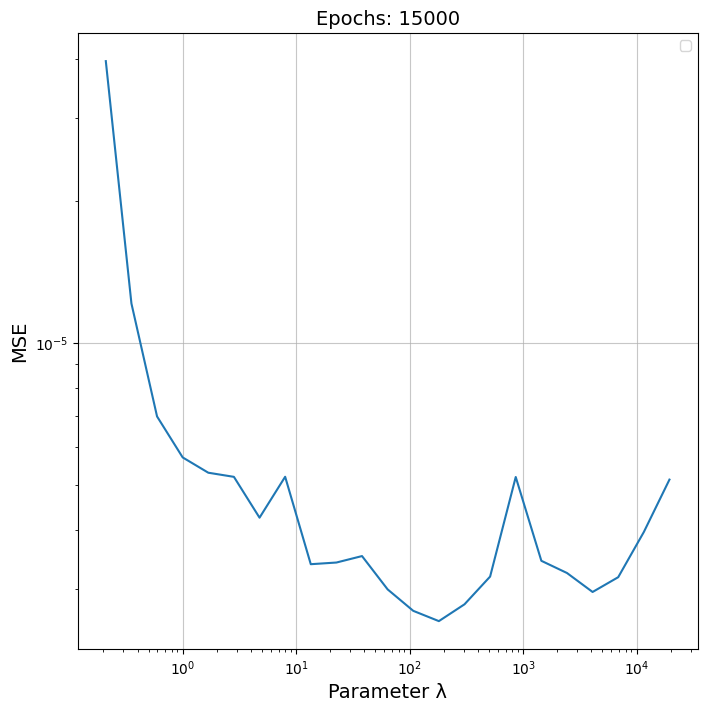
\includegraphics[height=7cm, keepaspectratio]{images/1.png}
    }
    \end{subfigure}
    \hfill
    \begin{subfigure}{0.45\textwidth}{
        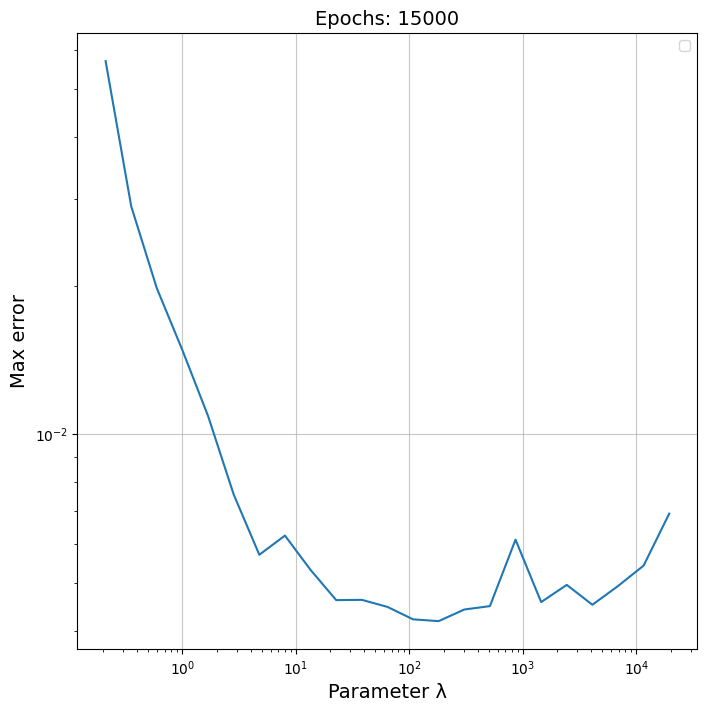
\includegraphics[height=7cm, keepaspectratio]{images/2.png}
    }
    \end{subfigure}
    \caption{15000 эпох, среднеквадратичная и максимальная ошибка}
\end{figure}

Точные цифры привести, к сожалению, не приведены. Но ошибка, будет видно позже по тепловой карте, не превышает $5e-3$.

\begin{figure}[ht!]
    \centering
    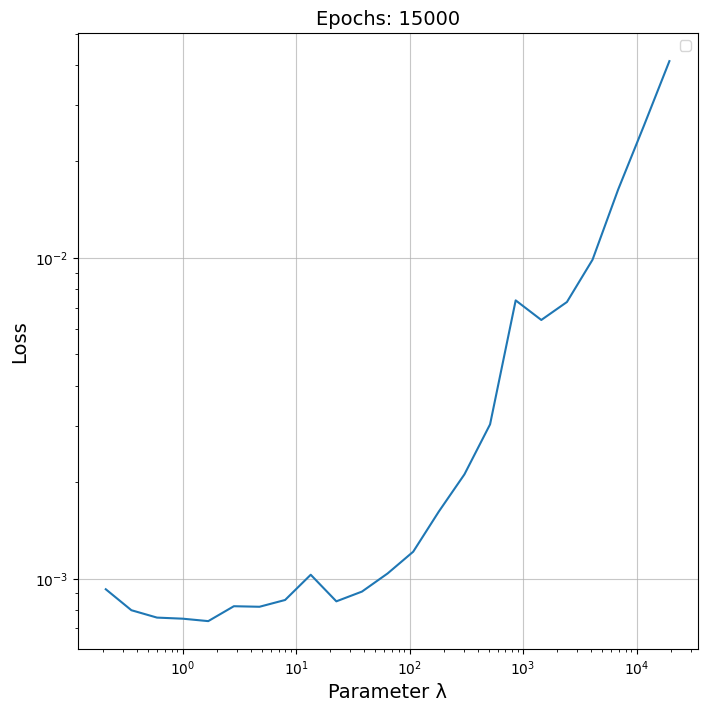
\includegraphics[width=0.45\hsize]{images/6.png}
    \caption{15000 эпох, потери, сходимость}
\end{figure}

\newpage

Можно сделать, очевидный вывод о том, что меньшее значение функции потерь необязательно приводит к уменьшению ошибки аппроксимации.
Очевидный в силу того, что для больших лямбда функция $L(\omega, \lambda)$ больше из-за роста множителя при второй сумме.


\begin{figure}[ht!]
    \centering
    \begin{subfigure}{0.4\textwidth}{
        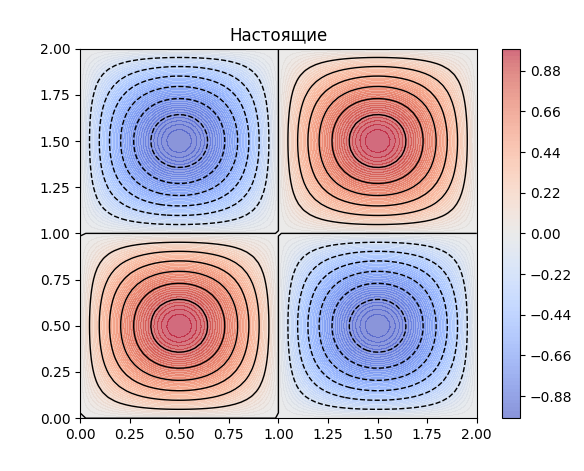
\includegraphics[height=7cm, keepaspectratio]{images/3.png}
    }
    \end{subfigure}
    \hfill
    \begin{subfigure}{0.4\textwidth}{
        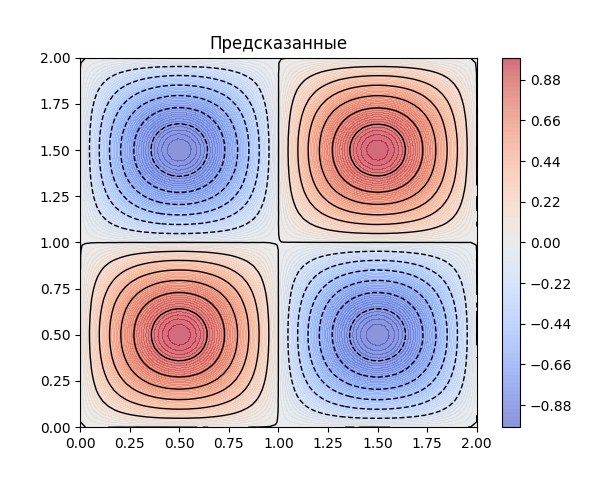
\includegraphics[height=7cm, keepaspectratio]{images/4.png}
    }
    \end{subfigure}
    \caption{Тепловая карта настоящей функции и значений модели (гиперпараметр неизвестен)}
\end{figure}

\begin{figure}[ht!]
    \centering
    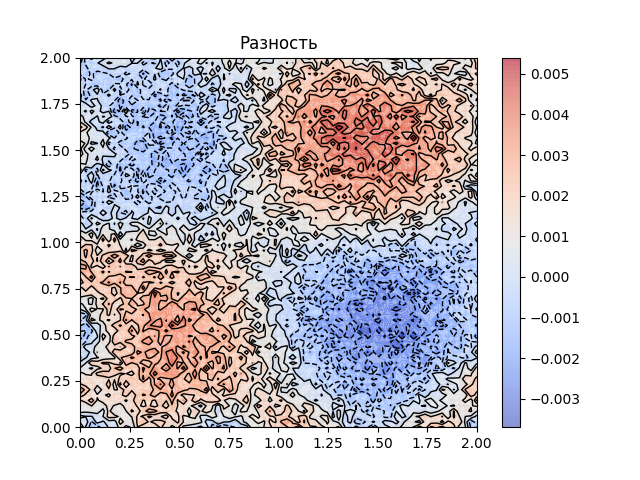
\includegraphics[width=0.75\hsize]{images/19.png}
    \caption{Разница приведенных сверху карт}
\end{figure}

Различие достаточно большое в рамках численных методов, но видно, что нейросеть приближает то, что нужно.

\newpage

В качестве дополнительных проверок была сделана небольшая визуализация сечения решений и графики ошибки на разных частях $\Omega$.

\begin{figure}[ht!]
    \centering
    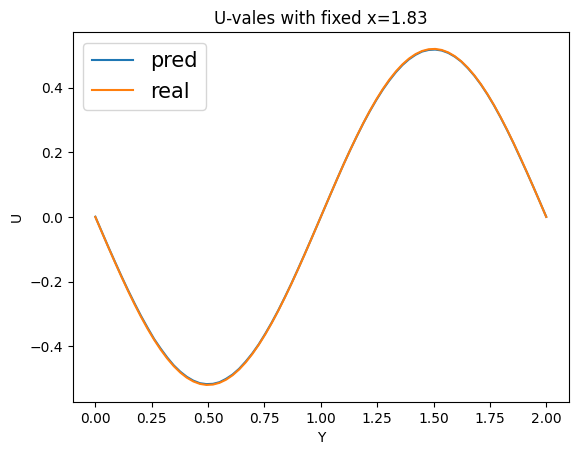
\includegraphics[width=0.75\hsize]{images/5.png}
    \caption{Сечение $u(x, y)$ и $NN(x, y)$ при $x = 1.83$}
\end{figure}

Видно, что разница между между графиками небольшая.

\begin{figure}[ht!]
    \centering
    \begin{subfigure}{0.45\textwidth}{
        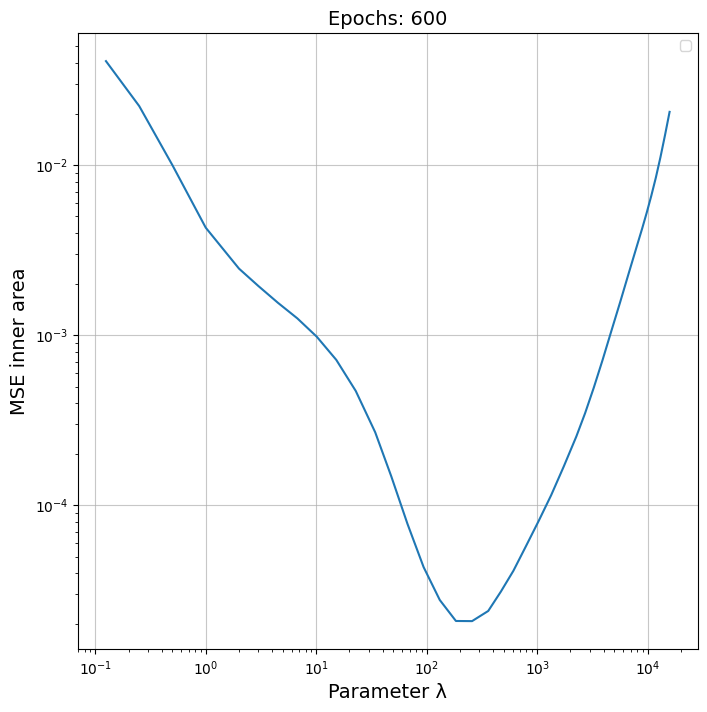
\includegraphics[height=8.5cm, keepaspectratio]{images/8.png}
    }
    \end{subfigure}
    \hfill
    \begin{subfigure}{0.45\textwidth}{
        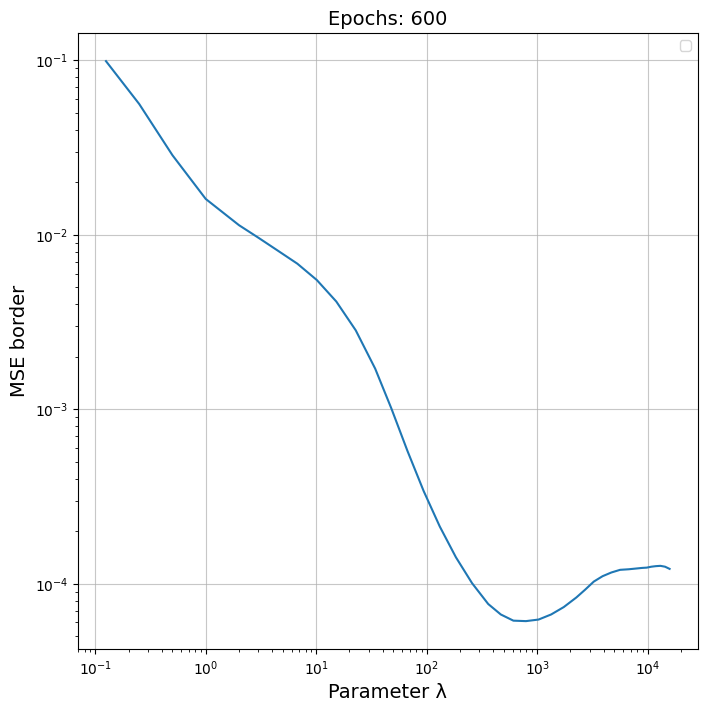
\includegraphics[height=8.5cm, keepaspectratio]{images/9.png}
    }
    \end{subfigure}
    \caption{Ошибка на $int(\Omega)$ и $\partial \Omega$ при 600 эпохах}
\end{figure}

\begin{figure}[ht!]
    \centering
    \begin{subfigure}{0.45\textwidth}{
        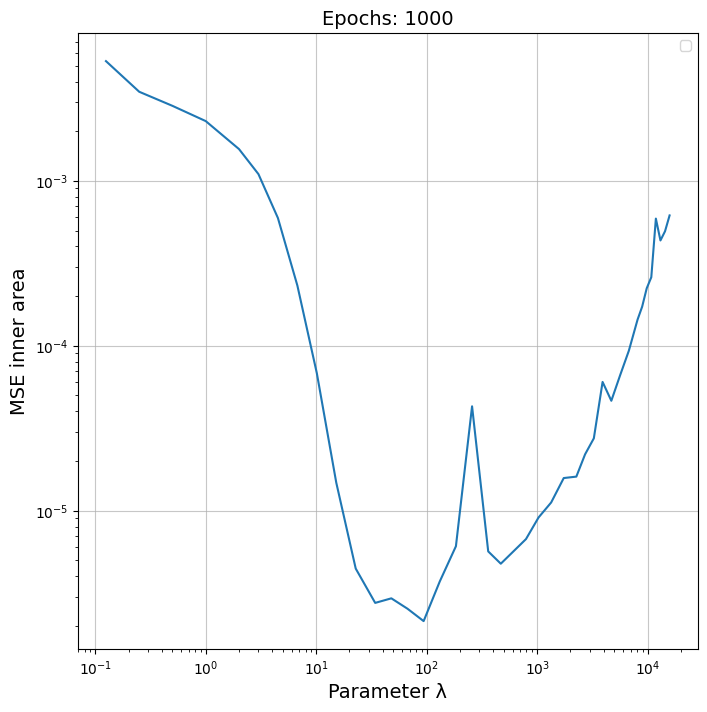
\includegraphics[height=8.5cm, keepaspectratio]{images/10.png}
    }
    \end{subfigure}
    \hfill
    \begin{subfigure}{0.45\textwidth}{
        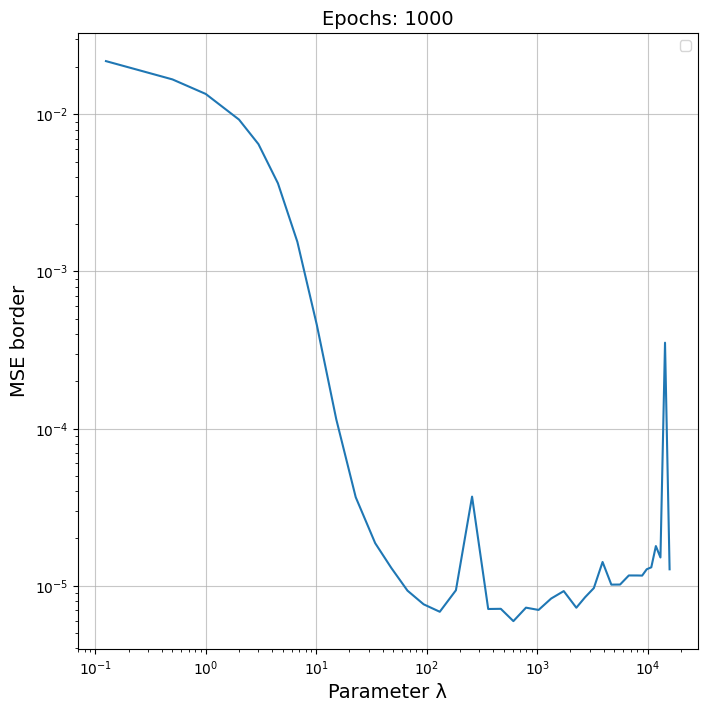
\includegraphics[height=8.5cm, keepaspectratio]{images/11.png}
    }
    \end{subfigure}
    \caption{Ошибка на $int(\Omega)$ и $\partial \Omega$ при 1000 эпох}
\end{figure}

Работа функции потерь подтверждается, так как при больших значениях гиперпараметра ошибка на границе растет слабее, 
чем внутри множества, в силу стремления нейросети минимизировать функцию потерь, в которую как раз наибольший вклад дает 
ошибка на границе.

\newpage

Интересно было узнать, есть ли такое предельное значение для количества эпох, в течение которых тренируется модель, 
что гиперпараметр перестает влиять на ошибку. Поэтому для той же модели, что и раньше, мы решили проверить это.

\begin{figure}[ht!]
    \centering
    \begin{subfigure}{0.45\textwidth}{
        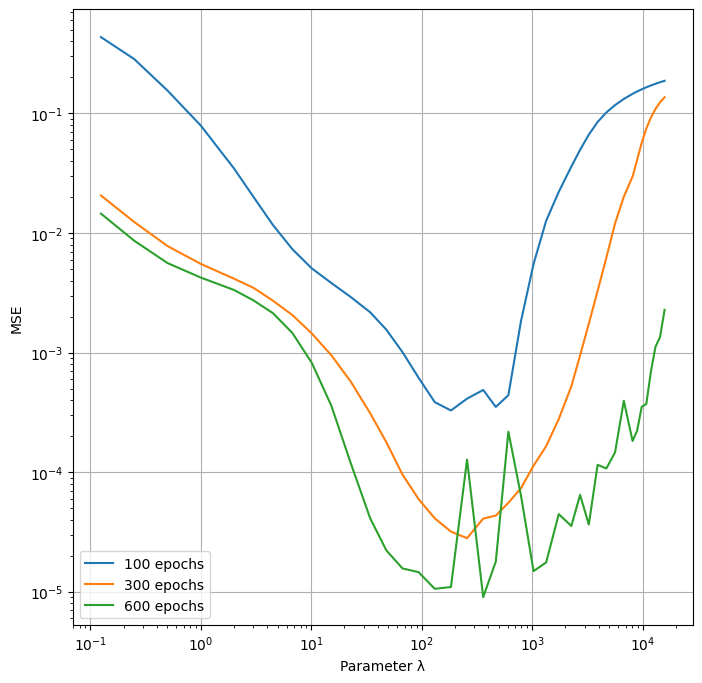
\includegraphics[height=8.5cm, keepaspectratio]{images/7.png}
    }
    \end{subfigure}
    \hfill
    \begin{subfigure}{0.45\textwidth}{
        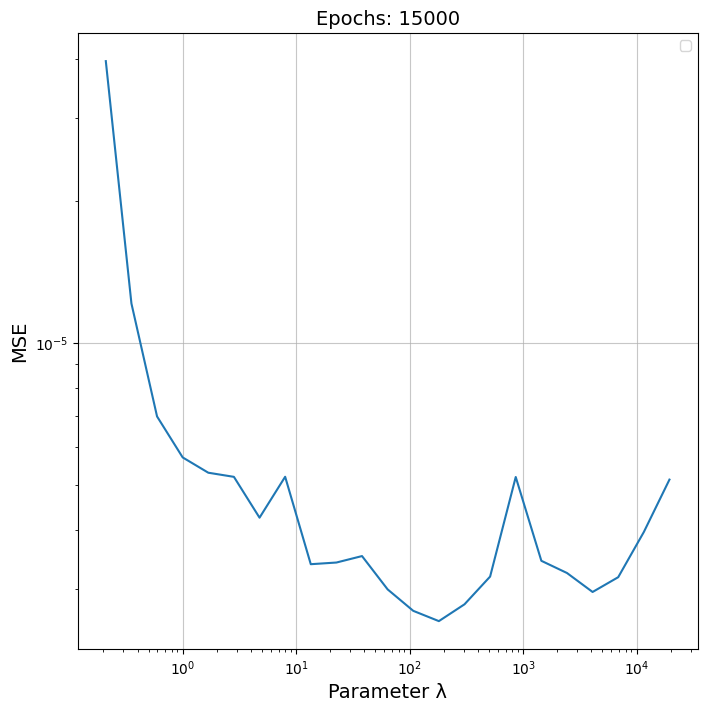
\includegraphics[height=8.5cm, keepaspectratio]{images/1.png}
    }
    \end{subfigure}
    \caption{Малое и большое число эпох, графики ошибки}
\end{figure}

Видно, что динамика на меньшую ошибку при $\lambda \in [10^2, 10^3]$ сохраняется, несмотря на "тренированность" модели.
Можно сделать $\textbf{вывод}$: неважно сколько вы будете тренировать модель, с правильным гиперпараметром она будет всегда выдывать лучший результаты.

\newpage

Также любопытно, как связаны размер модели, значение гиперпараметра и ошибка. Например, справедливо ли утверждение: для легкой модели выбор правильного гиперпараметра менее важен?
Или для всех моделей сохраняется одинаковое поведение ошибки, как например было с разным числом эпох.

Мы сделали тесты на 4 моделях. Вот архитектуры 3х дополнительных моделей, помимо той, которая была представлена ранее.

\begin{figure}[ht!]
    \centering
    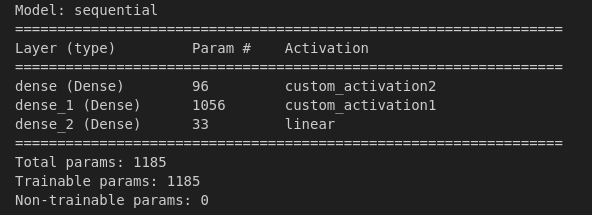
\includegraphics[height=4.5cm, keepaspectratio]{images/16.png}
    \caption{Модель с 2 внутренними слоями}
\end{figure}

\begin{figure}[ht!]
    \centering
    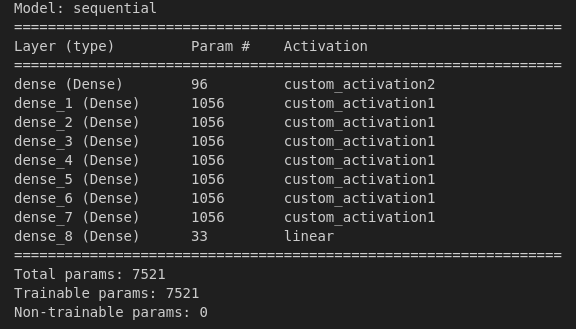
\includegraphics[height=4.5cm, keepaspectratio]{images/17.png}
    \caption{Модель с 8 внутренними слоями}
\end{figure}

\begin{figure}[ht!]
    \centering
    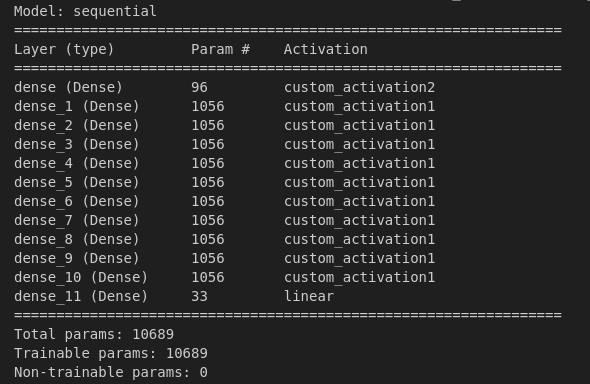
\includegraphics[height=4.5cm, keepaspectratio]{images/18.png}
    \caption{Модель с 11 внутренними слоями}
\end{figure}

Как видно, было просто увеличено количество внутренних слоев.

\begin{figure}[ht!]
    \centering
    \begin{subfigure}{0.45\textwidth}{
        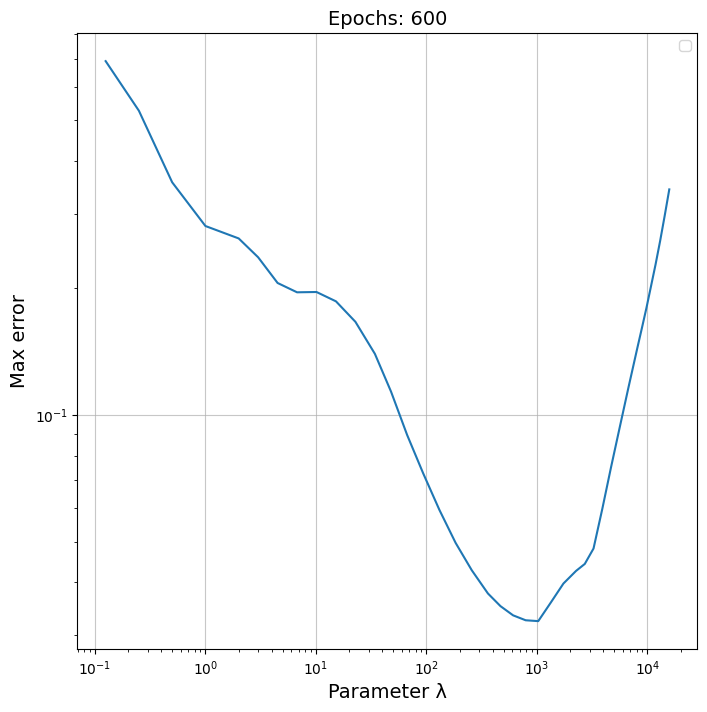
\includegraphics[height=7.5cm, keepaspectratio]{images/12.png}
    }
    \end{subfigure}
    \hfill
    \begin{subfigure}{0.45\textwidth}{
        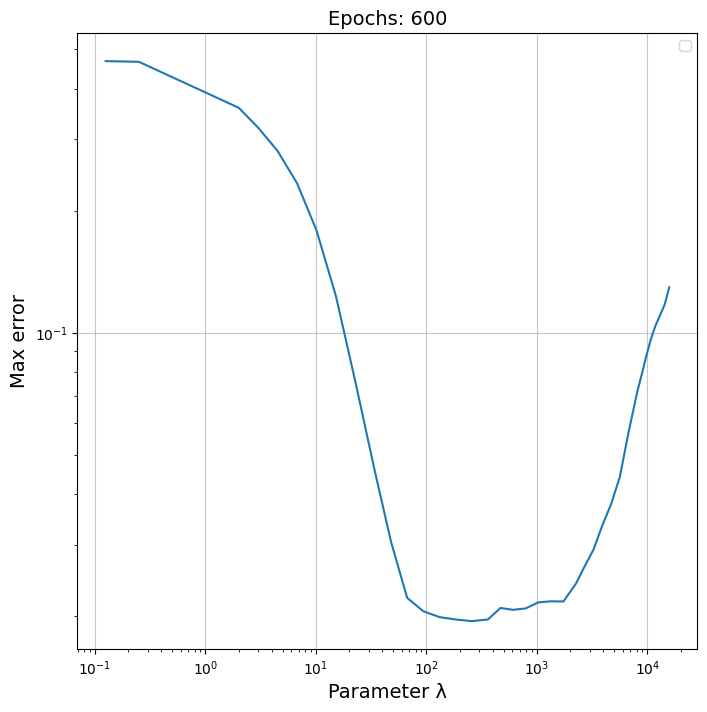
\includegraphics[height=7.5cm, keepaspectratio]{images/13.png}
    }
    \end{subfigure}
    \caption{Результаты тестов 1}
\end{figure}

\begin{figure}[ht!]
    \centering
    \begin{subfigure}{0.45\textwidth}{
        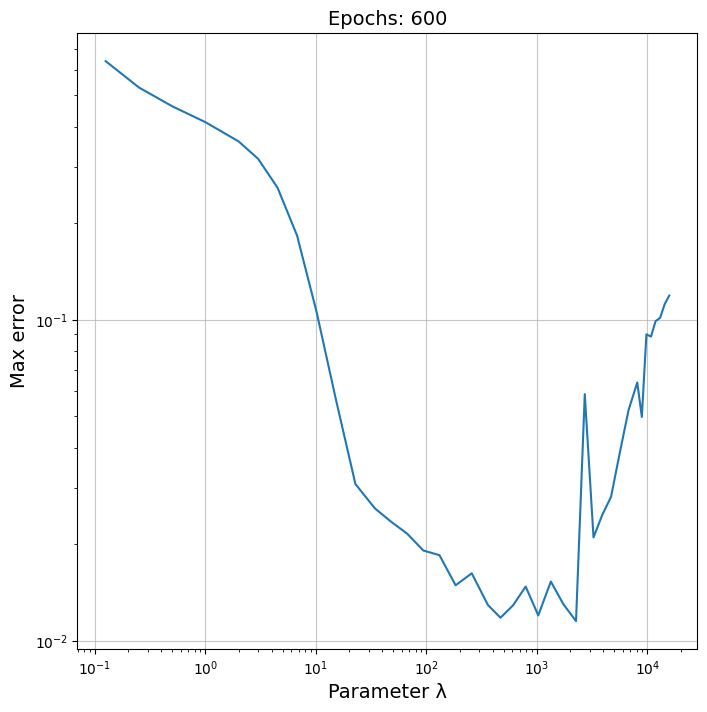
\includegraphics[height=7.5cm, keepaspectratio]{images/14.png}
    }
    \end{subfigure}
    \hfill
    \begin{subfigure}{0.45\textwidth}{
        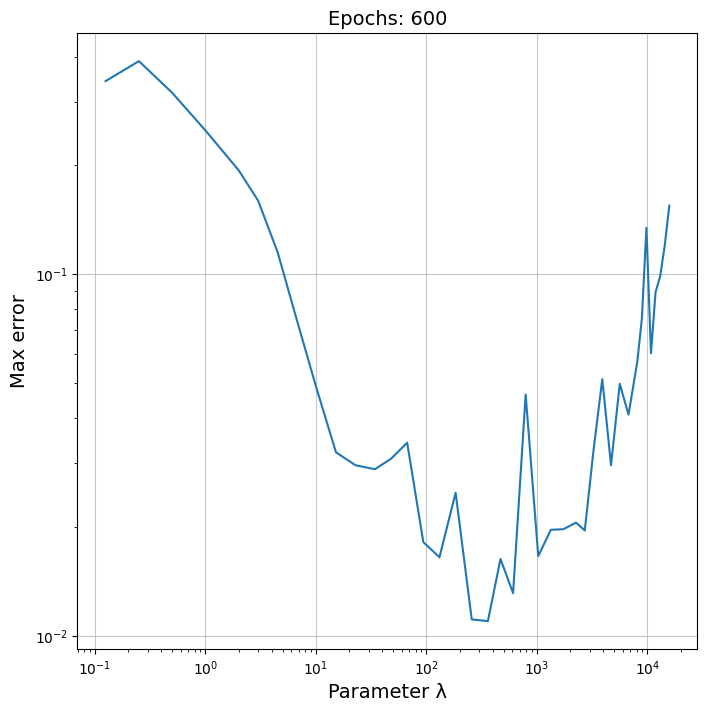
\includegraphics[height=7.5cm, keepaspectratio]{images/15.png}
    }
    \end{subfigure}
    \caption{Результаты тестов 2}
\end{figure}

Картинки идут в порядке возрастания количества параметров у моделей. Видно, что у больших моделей, видимо в силу их "гибкости" 
влияние гиперпараметра становится слабее, при примерно такой ошибке, т.е. $\lambda$, "выравнивая" ошибку, не увеличивает ее.

Конечно нужно делать гораздо больше тестов, проверять другие функции, а главное новые гипотезы. Поэтому проекту есть куда расти и развиваться.

\newpage
